%% -*- coding:utf-8 -*-
\begin{figure}
\centering

\ifpdf
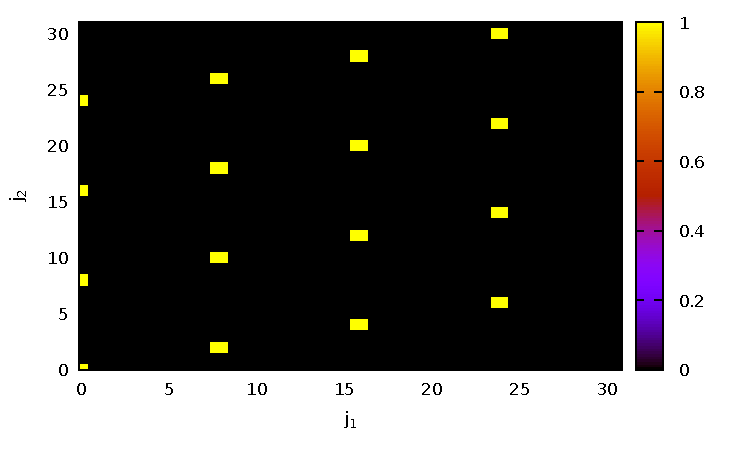
\includegraphics[angle=0]
{./part4/quantcomp/picdiscretlog2.pdf}
\else
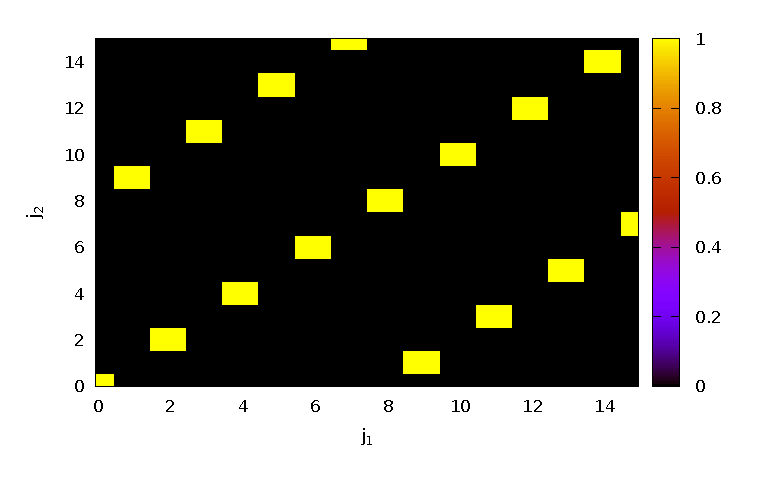
\includegraphics[angle=0]
{./part4/quantcomp/picdiscretlog2.eps}
\fi

%\input ./part4/quantcomp/picdiscretlog2.tex

\caption{Фурье образ функции с \autoref{fig:part4:quantcomp:dl1}.
  Число отсчетов $M=32$. Период по координате $j_1$ $T_{j_1} = 8$, что
соответствует периоду по оригинальной координате $t_1 =
\frac{M}{T_{j_1}} = 4$. Период по координате $j_2$ $T_{j_2} = 2$, что
соответствует периоду по оригинальной координате $t_2 =
\frac{M}{T_{j_2}} = 16$. Решением уравнения $3^x \equiv 13 \mod 17$
является $x = \frac{16}{4} = 4$} 
\label{fig:part4:quantcomp:dl2}
\end{figure}
